\chapter{Runway design}

	\section{Runway 1}
	\paragraph{} B777-300ER and A330-300, are found to be the bigger planes with higher requirements to operate on the new airport. Comparing both aircrafts, the B777-300ER is the most restrictive one, with an MTOW of 350.000Kg versus the 233.000kg of MTOW of the A330-300.
	
	The dimensions of the aircraft are the following:
	
	\begin{figure}[H]
		\centering
		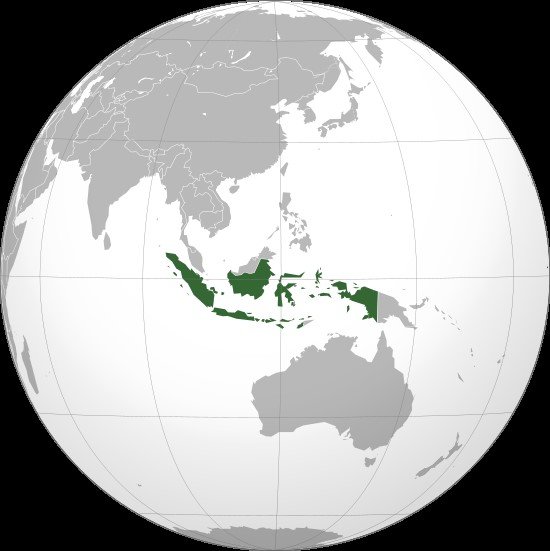
\includegraphics[clip, trim=0cm 0cm 0cm 0cm, width=1\textwidth]{./images/RUNWAY_DSGN/mainPlane}
		\caption{Main plane.} %nom de la figura
		\label{main_plane} %per denotar una referencia
	\end{figure}

%per fer referencies
	Fig. \ref{main_plane}
	
	
	\begin{table}[htb]
		\centering
		\begin{tabular}{ll p{5cm}}
			\toprule[2pt]
			\textbf{Features} &   \\
			\midrule[1pt]
			Voltage& 14.8V\\
			Type& LiPo 4S1P\\
			Max. continuous discharge & 20C (100A) \\
			Charging current& 4C (20A)\\
			Weight& 499g\\
			Connectors& XT60, JST-XH(balancing)\\
			\bottomrule[2pt]
		\end{tabular}
		\caption{LiPo 4S 5000mAh 20-40C SLS XTRON}
		\label{featuresBattery}
	\end{table}
	
	\section{Runway length}
		\subsection{Runway length for reference aircraft}
		\subsection{Final runway length}
		
	\section{Runway width}
		\subsection{Runway width for reference aircraft}
		\subsection{Final runway width}
		
	\section{Reference code}
	
	\section{Declared distances}
	
	\section{Protection and safety areas}
		\subsection{Runway shoulders}
		\subsection{Runway strips}
		\subsection{Runway end safety area (RESA)}
		\subsection{Stopway (SWY)}
		\subsection{Clearway (CWY)}
		